\section{Visual Object Tracking}

% -------------------------------------------------------------------------------------------------
\subsection{OTB 2013 and 2015}
\label{ssec:DatasetOTB1315}

\todo[inline]{Add OTB2013 and 2015 summary.}

% -------------------------------------------------------------------------------------------------
\subsection{GOT10k}
\label{ssec:DatasetGOT10k}

\todo[inline]{Add GOT10k summary.}

% -------------------------------------------------------------------------------------------------
\subsection{VOT 2019}
\label{ssec:DatasetVOT2019}

\todo[inline]{Talk about variations (years 2015, 2016, 2018, 2019).}

This prominent dataset (web: \cite{vot2019dataset}) is a benchmark in visual object tracking \cite{Kristan2019a}. It has a long history of development and annual challenges for the best visual tracker. All \datasetname{\gls{vot} 2019} datasets are available through the \gls{vot} toolkit. The pipeline for evaluating a tracker is automated to facilitate ease of use and a framework for researchers to allow an objective comparison with others. The dataset provides multiple video sequences where a single object is present under various conditions. For example, people running, a fish swimming behind corals, a vehicle driving in a city, and so forth. Each object is annotated by a single \gls{bbox} per each frame in which it appears.

% -------------------------------------------------------------------------------------------------
\subsection{KITTI Object Tracking}
\label{ssec:DatasetKITTIObjectTracking}

This object tracking benchmark \cite{Geiger2012CVPR} (web: \cite{kittiobjecttrackingdataset}) consists of $21$ training sequences and $29$ test sequences. Even though there have been labeled $8$ different classes, only the classes "car" and "Pedestrian" are evaluated in this benchmark, as only for those classes enough instances for a comprehensive evaluation have been labeled. Considering our potential traffic application, this fact does not represent a disadvantage. The goal in the object tracking task in this benchmark is to estimate object tracklets for the classes "car" and "pedestrian". Only $2D$ $0$-based, axis-aligned \glspl{bbox} in each image are evaluated.

\begin{figure}[t]
    \centerline{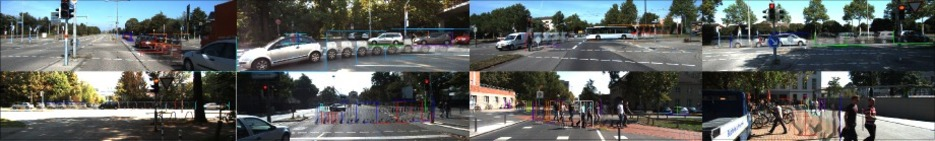
\includegraphics[width=\linewidth]{figures/datasets/kitti_object_tracking_sample.jpg}}
    \caption[\datasetname{KITTI Object Tracking} dataset]{A sample of the only two classes ("car" and "pedestrian") that are evaluated in the benchmark using the \datasetname{KITTI Object Tracking} dataset. \externalsrc{\cite{kittiobjecttrackingdataset}}}
    \label{fig:DatasetKITTIObjectTracking}
\end{figure}

% -------------------------------------------------------------------------------------------------
\subsection{UA-DETRAC}
\label{ssec:DatasetUADETRAC}

The most important benchmark dataset for our work is \datasetname{UA-DETRAC} \cite{CVIU_UA-DETRAC} (web: \cite{uadetracdataset}). To the best of our knowledge, this dataset the most favorably suits our needs of all surveyed datasets available. The primary reason is that is provides a plethora of traffic situations recorded using a static camera (see Fig.~\ref{fig:DatasetUADETRAC}). This setup appropriately reflects the requirements of our goal, which is the analysis of traffic scenes using object tracking algorithms. This work provides high quality human-generated annotations with a lot of additional information about the captured vehicles, such as the intensity of their occlusion. Among other things, we treat this benchmark as the base of our experiments even thanks to the existence of online leaderboard, which provides an the opportunity to compare our solution with others using the same metrics.

\datasetname{UA-DETRAC} is considered a challenging real-world multi-object detection and multi-object tracking benchmark. The dataset consists of $10$ hours of videos captured at $24$ different locations in China. The videos are recorded at $25$ \gls{fps}, with resolution of $960 \times 540$ pixels. There are more than $140\ 000$ frames and $8\ 250$ vehicles that are manually annotated, leading to a total of $1.21$ million labeled \glspl{bbox} of objects.

\begin{figure}[t]
    \centerline{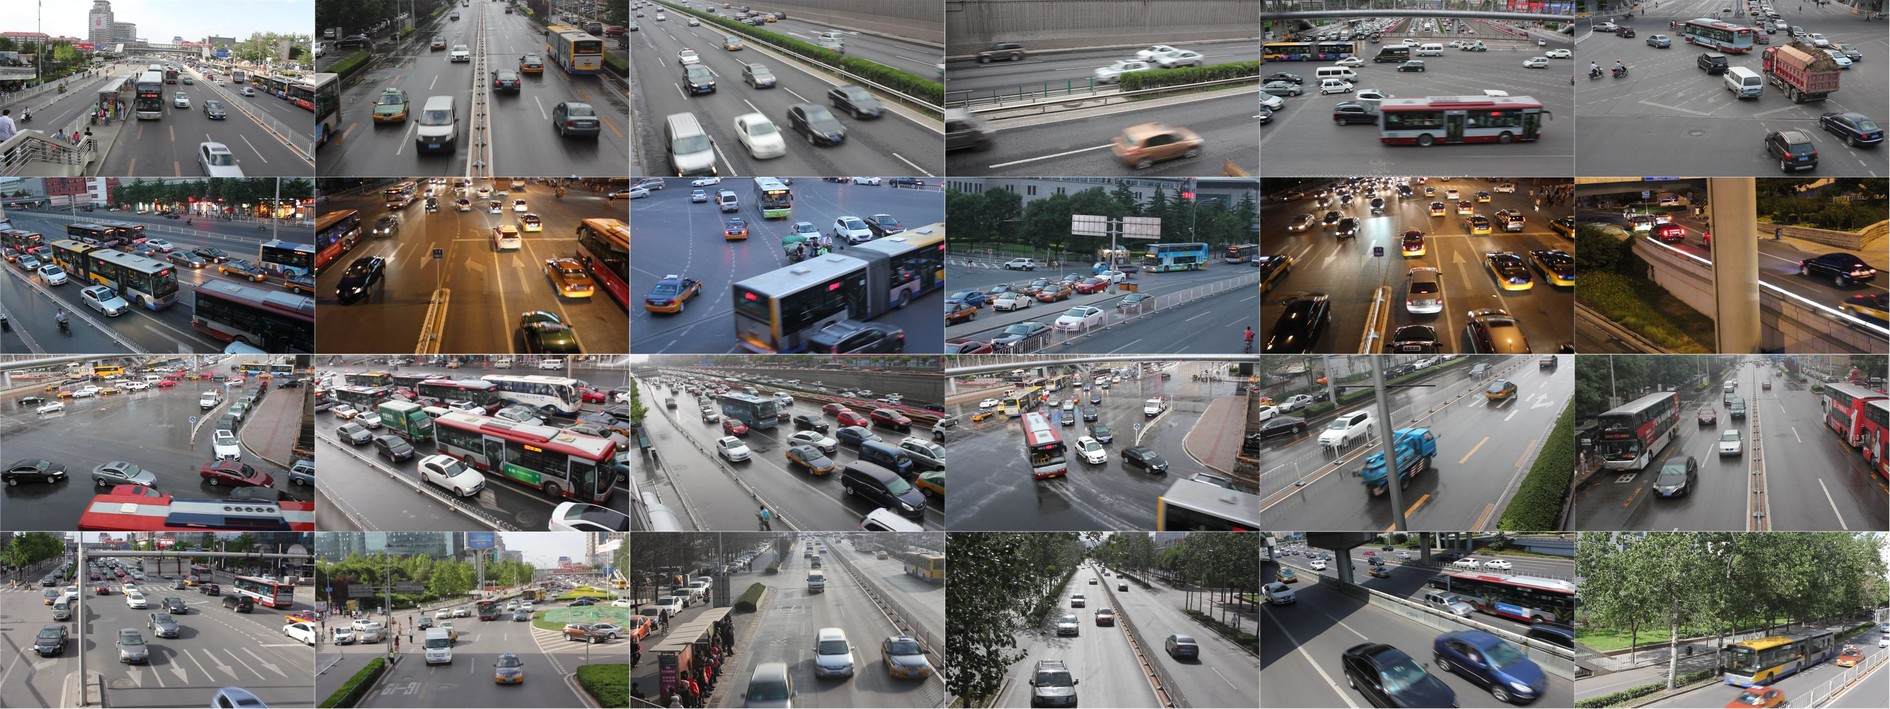
\includegraphics[width=\linewidth]{figures/datasets/uadetrac_samples.jpg}}
    \caption[\datasetname{UA-DETRAC} dataset]{A sample from the \datasetname{UA-DETRAC} dataset. The whole dataset consists of diverse traffic situations captured using a static camera viewed from various angles. \externalsrc{\cite{uadetracdataset}}}
    \label{fig:DatasetUADETRAC}
\end{figure}

\def\uadetracfigsize{0.4}

\begin{figure}[t]
    \centering
    \begin{subfigure}[b]{\uadetracfigsize\textwidth}
        \centering
        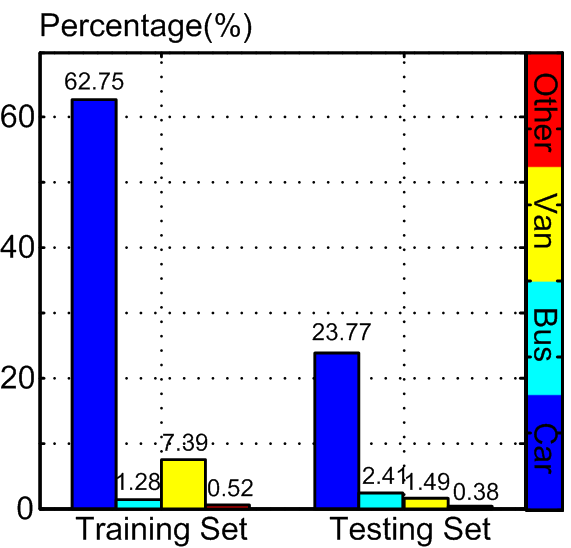
\includegraphics[width=\textwidth]{figures/datasets/uadetrac_stats_vehicle_category.png}
        \caption[]{}
    \end{subfigure}
    \hfill
    \begin{subfigure}[b]{\uadetracfigsize\textwidth}
        \centering
        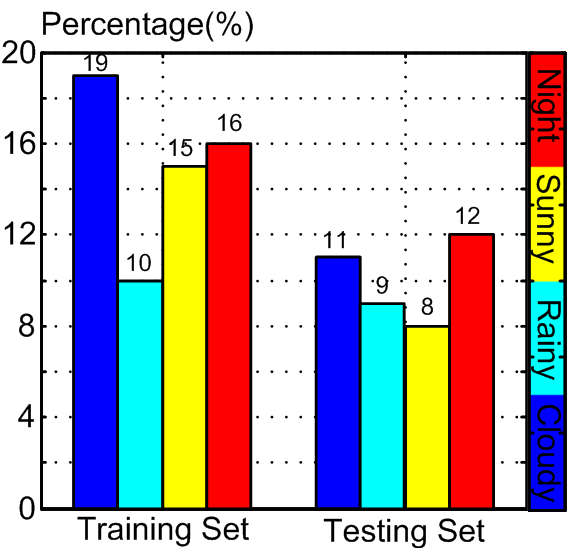
\includegraphics[width=\textwidth]{figures/datasets/uadetrac_stats_weather.png}
        \caption[]{}
    \end{subfigure}
    \hfill
    \begin{subfigure}[b]{\uadetracfigsize\textwidth}
        \centering
        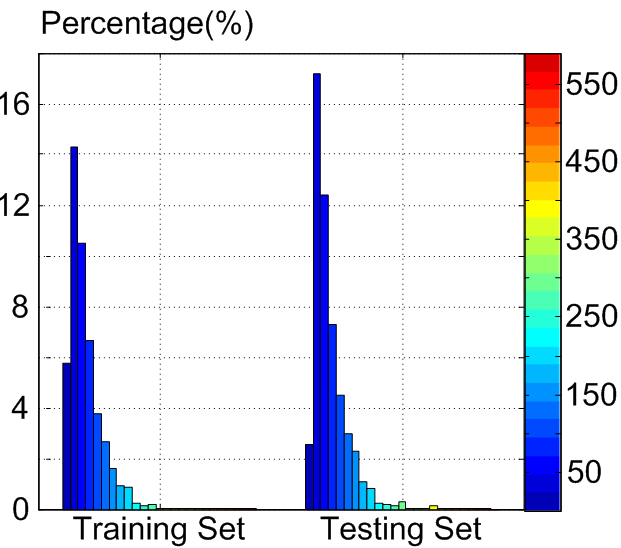
\includegraphics[width=\textwidth]{figures/datasets/uadetrac_stats_scale.png}
        \caption[]{}
    \end{subfigure}
    \hfill
    \begin{subfigure}[b]{\uadetracfigsize\textwidth}
        \centering
        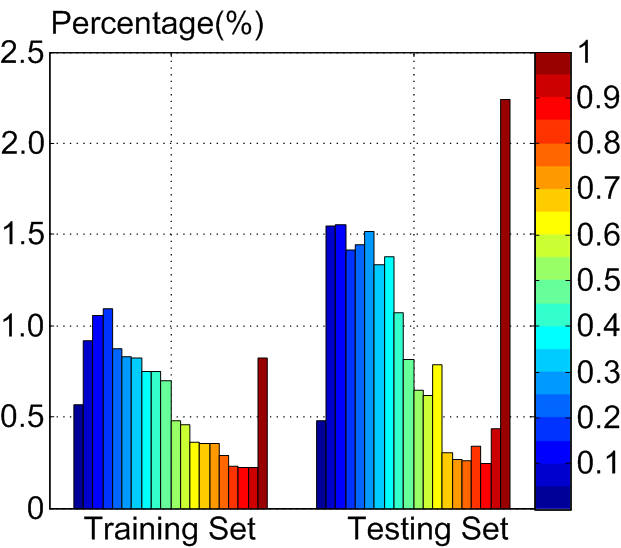
\includegraphics[width=\textwidth]{figures/datasets/uadetrac_stats_occlusion_ratio.png}
        \caption[]{}
    \end{subfigure}
    \caption[\datasetname{UA-DETRAC} dataset overview]{Summary statistics of the \datasetname{UA-DETRAC} dataset. Subfigure (a) shows the distribution of vehicle categories, one of \emph{car}, \emph{bus}, \emph{van} or \emph{other}; (b) shows the varying weather conditions belonging to either \emph{night}, \emph{sunny}, \emph{rainy} or \emph{cloudy}; (c) depicts the change in scale given by the square root of the \gls{bbox} pixel area; and (d) reflects the occlusion ratio throughout the dataset computed as the fraction of the vehicle \gls{bbox} being occluded . \externalsrc{\cite{uadetracdataset}}}
    \label{fig:UADETRACStats}
\end{figure}

Since this dataset is of paramount importance to our research, here we provide more details about the structure and properties of the contained data compared to other datasets described in our work. The dataset consists of $100$ videos, where $60$ of them are dedicated to training, while the remaining $40$ are used for testing. Ground-truth annotations are provided in both variations. This is not always the case, as several benchmarks do not disclose annotations for the test dataset, e.g., \datasetname{KITTI} \cite{Geiger2012CVPR}.

\begin{figure}[t]
    \centerline{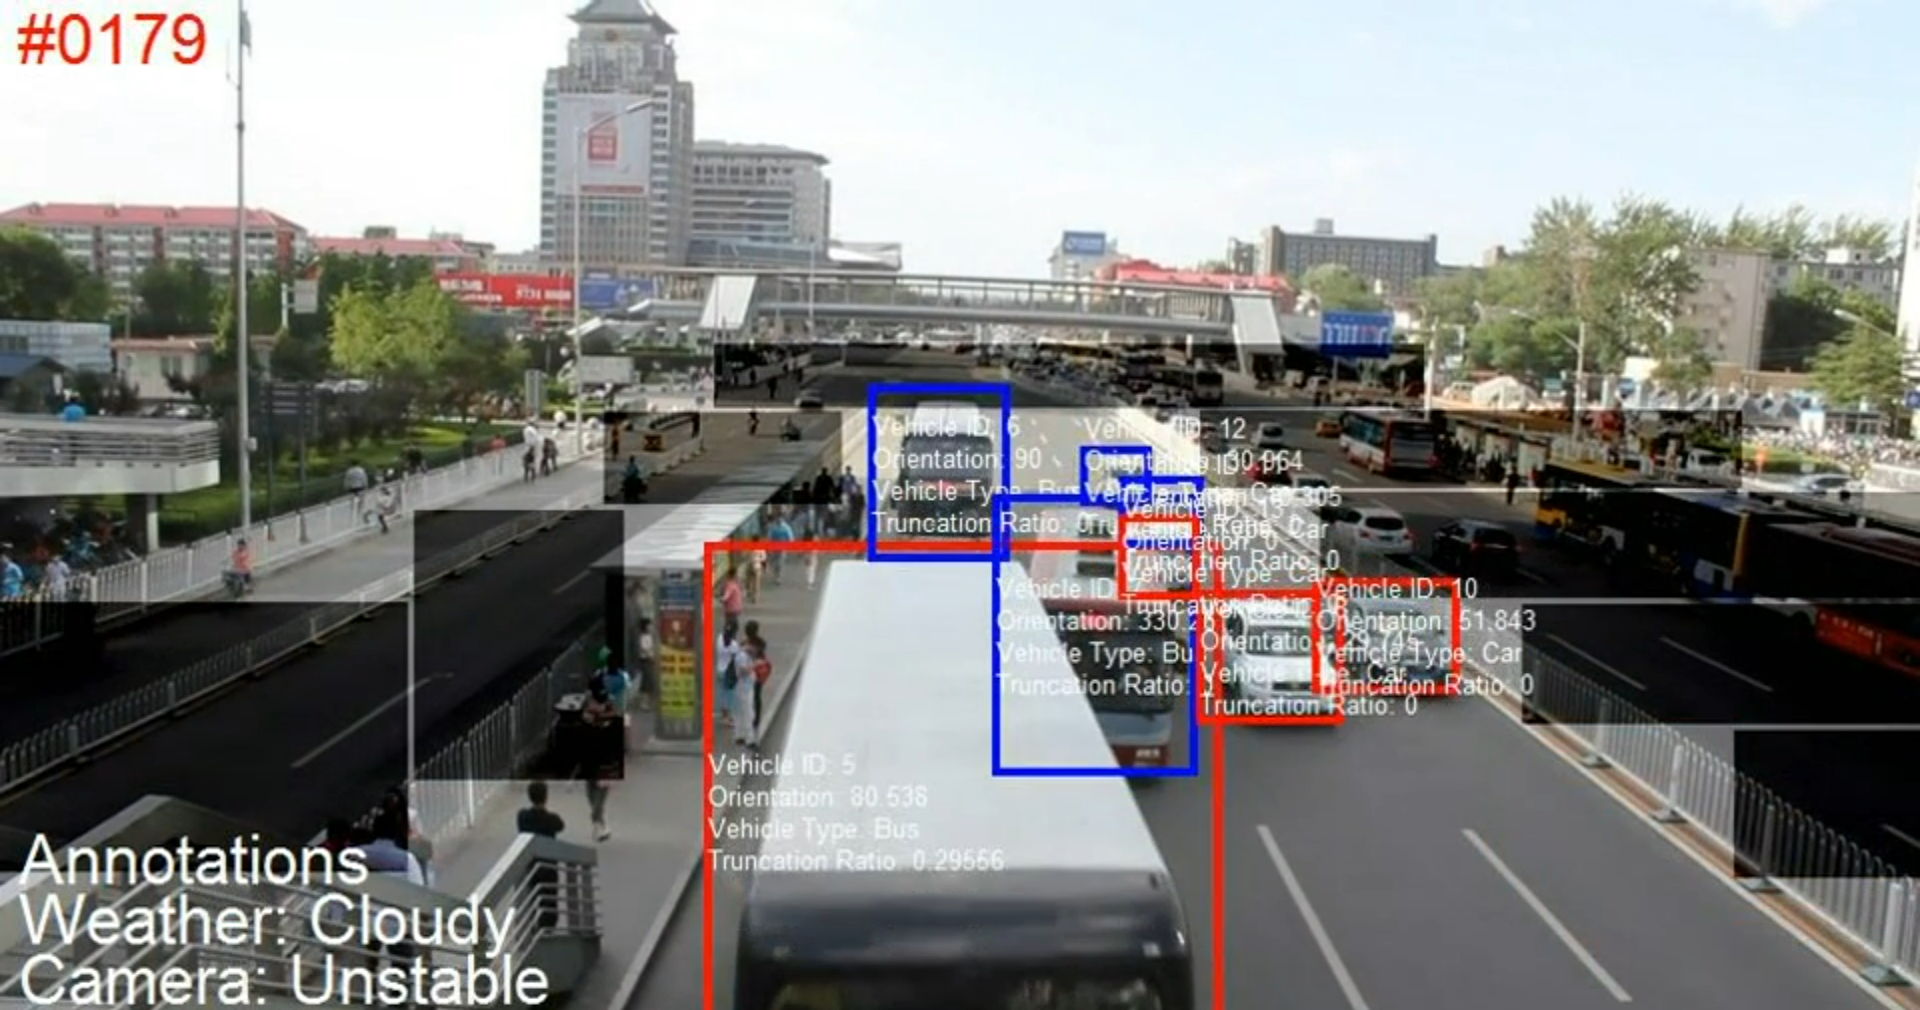
\includegraphics[width=0.8\linewidth]{figures/datasets/uadetrac_ignored_regions.png}}
    \caption[Ignored regions in \datasetname{UA-DETRAC}]{A demonstration of a possible distribution of ignored regions in the \datasetname{UA-DETRAC} dataset. \externalsrc{\cite{uadetracdataset}}}
    \label{fig:UADETRACIgnoredRegions}
\end{figure}

The dataset author's provide extensive information about vehicle, including its speed in frames per second, color, orientation, and occlusion. Due to space restrictions, we limit our elaboration on how the data was obtained only to the fields pertinent to our usage. At the beginning, there is a section describing some ignored regions (see Fig.~\ref{fig:UADETRACIgnoredRegions}). The authors decided to omit regions with very dense traffic. Nevertheless, the dataset contains a plethora of scenes where the number of cars is very high. More specifically, Table~ describes some basci statistical properties of the distribution of the number of cars throughout the dataset. The data were obtained by collecting the number of annotated cars for each frame. Training and testing data were merged for simplicity.
